\documentclass[11pt]{article}

\usepackage{graphicx, epsfig}
\usepackage{amsmath, amssymb, latexsym}
\usepackage[english]{babel}
\usepackage{amssymb}   
%\usepackage{graphicx}
%\usepackage{float} 






% Make a larger page (shrink the margins)
%
\setlength{\textwidth}{6.7in}
\setlength{\textheight}{9.0in}
\setlength{\evensidemargin}{0.0in}
\setlength{\oddsidemargin}{0.0in}
\topmargin -0.5in
\footskip 0.5in



\title{Progress Report}
\author{Eric Davis}
\begin{document}
\maketitle
\medskip



\section{Column Profiles}
\hspace{0.5cm}

Much of the week was spent trying to find stars to perform an analysis on. To do this I continue to view nights in at most three hour chunks. However, one of the big problems for locating stars is they tend to radiate at about 300-500 counts per bin. Unfortunately on most nights clouds will radiate at about the same rate, which means stars are essentially indistinguishable from background noise. Again, I can't see any shortcuts to expedite the process besides physically examining data a night at a time. I have started to produce tables of Gaussian values. Although the plots produce last week were decent, they contained a lot of noise. Playing around to get the best results I found averaging the column counts over the star flattened the noise and tended to produce a smoother Gaussian shape. I think this will provide the most accurate method for pinpointed exact transit times and locations of stars. 


\begin{figure}[h!]
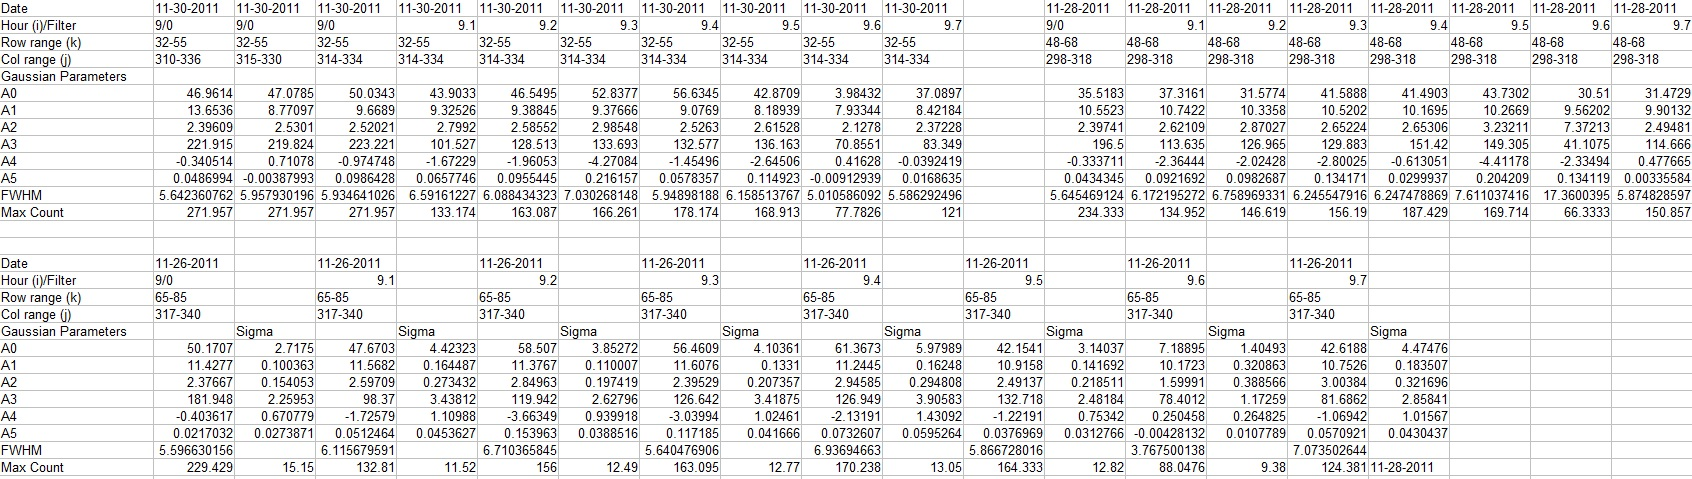
\includegraphics[scale=0.4]{star_profile_spreadsheet.jpg}
\caption{The location and Gaussian parameters of a sample star over several nights. This also compares the different filters for the same star. The most pronounced of all filters was the red (0) filter, demonstrated by consistently having the highest peak counts.}
\end{figure}


\begin{figure}[h!]
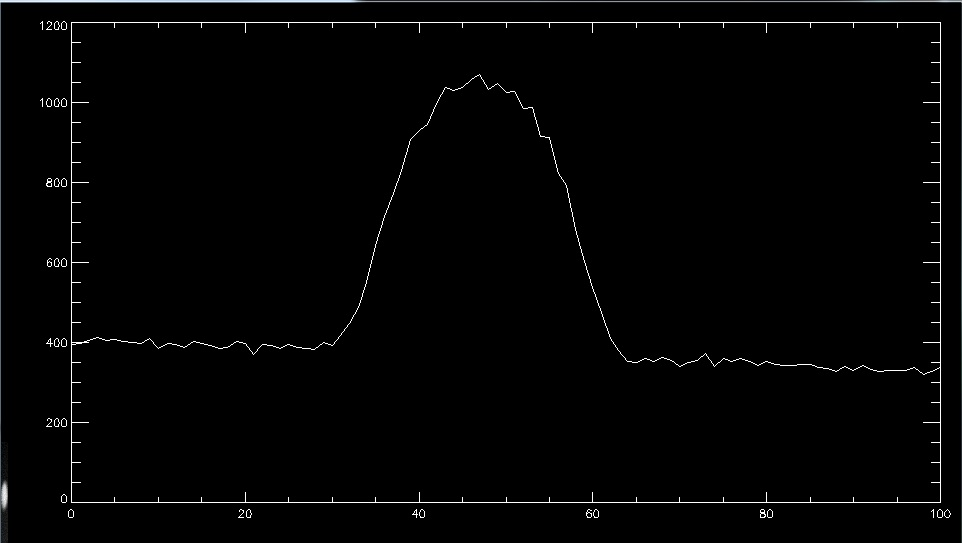
\includegraphics[scale=0.7]{jupiter_line_plot.jpg}
\caption{This is an averaged row profile of Jupiter from November 6, 2011. The same data was used to produce the image in the bottom left corner of the figure. It is very much a Gaussian shape, and as discussed above the averaging process tends to smooth the background noise considerably. Note that even in this plot the background is radiating around 400 counts/bin }
\end{figure}


\section{Row Profiles}

After talking to you we discussed trying to take some profiles of Jupiter, as it radiates at a much higher rate than a star from our perspective. The downside is planets move much, much quicker than a star in our sky. However, I wrote a code that allows a user to fairly easily produce an averaged row profile of any section in the sky. It is quite robust in handling different sizes (heights,widths) of an image you wish to produce an averaged row profile, so much so that once an object is found it is a few clicks to get all of the information displayed in the spreadsheets. It helped to have a very similar script for the column profiles, and allowed me to touch up a few things that were inefficient or just annoying about the code I used for the column profiles. I am eager to start producing similar row profiles of the stars. Of course, the main bottleneck right now is finding them. 


\section{Future Considerations}

I want to get several more row profiles of Jupiter, and at the same time produce an averaged column profile of several nights to compare. However, the end goal is to find stars from several nights and apply the same process. As discussed, Jupiter is a good place to start to make sure the methodology is sound and we're getting the information we want out of the data. So again, I plan on spending most of my week tracking down the same star on different nights and continue to add to my data spreadsheets. As well, I would like to touch up my code for my column profile script with some tricks I learned for the row profile code.

\begin{figure}[t]
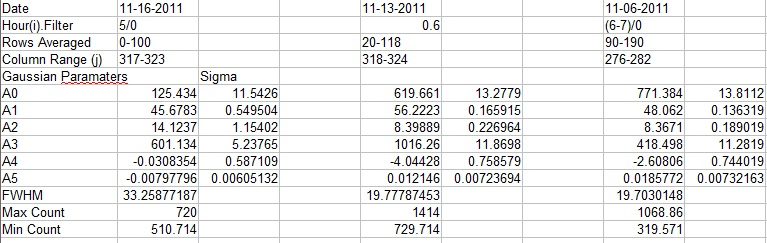
\includegraphics[scale=0.8]{jupiter_spreadsheet.jpg}
\caption{The parameters needed to produce an averaged row profile of Jupiter on different nights. As seen above, the different nights appear to have some very different parameters, particularly the night of the 16th.}
\end{figure}

\end{document}
\end{article}